\section{Variable Gain Amplifier}
The HMC694LPE Variable Gain Amplifier has 3 core inputs/outputs that are essential to operation: RF In, RF Out, and Control Voltage. RF In will be connected to the DRO's output and has a maximum power rating of 5 dBm, according to the datasheet. The gain is altered by the Control Voltage, meaning that we can control the amplitude of the carrier wave. Thus, we can create an effective amplitude modulator with these two alone. However, we must alter our given inputs to match the specifications of the variable gain amplifier. You already saw an example of this alteration with the DRO and RF In. Let us now see how the signal received by Control Voltage has been manipulated.

\subsection{Linear Region}\label{VGA Linear}
The linear region, that is, the region in which a change in control voltage will linearly change the gain in decibels, is between -1.35V and -1.07V, corresponding to a gain of 20dB and 8dB of gain, respectively. This is especially useful now, since we can predictably alter the message wave without too much effort. Given that we want modulation depth of $\pm$ 5dB, and that our positive amplitude of 1 should correspond to 5dB, we can select 15 dB of gain as our midpoint, a control voltage of -1.21V. Thus, calculating 5dB up results in 20 dB of gain, with a control voltage of -1.34V. However, the negative portion of the message is 56.3\% the size of its positive amplitude. Thus, our message should only reach -2.815dB from our calculated center point, or 12.185dBm, calculated from \(.563 * 5dB.\)

\begin{figure}[H]
    \centering
    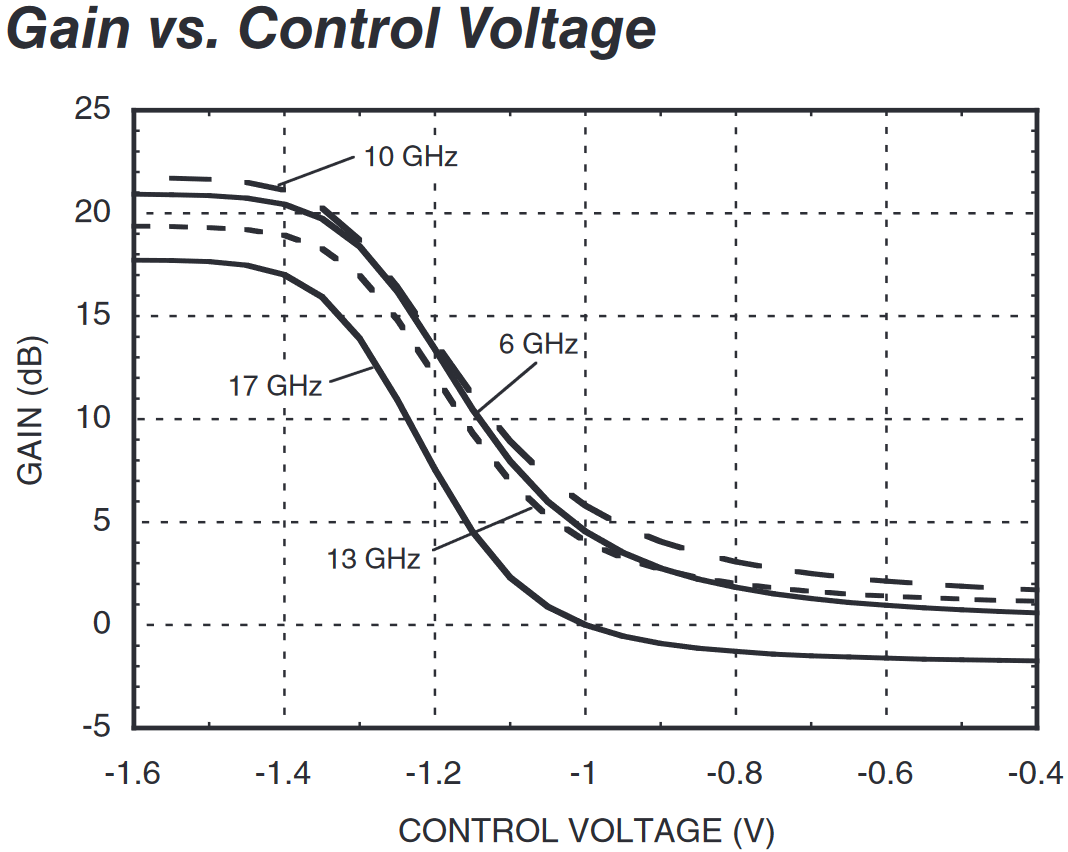
\includegraphics[width = 0.6\textwidth]{Images/Sub-figures_Example/Gain v Control Voltage.png}
    \caption{Gain vs Control Voltage of the HMC694LPE}
    \label{fig:my_label}
\end{figure}